\chapter{Preliminaries}

In this chapter the design considerations for the robot will be explained based on minimal required capabilities.
Two sources for energy harvesting will be compared based on average charge times.
Followed by an evaluation of two locomotion locomotion types considered for the transiently powered robot.
Finally, a simple model will capture the relation between power harvested and distance covered by the robot.

\section{Design Considerations}
\label{sec:design_considerations}

This section will shortly explain the main areas considered while designing the battery-less transiently-powered robot

% - Optimize or low power consumption (disable or standby sensors and motor ctrl when not used)
% - Minimal basic functionality (for simple swarm algorithms?) (but no power hungry components ie optical encoders or mouse sensors)
% - Low power communication
% - Navigation

% Extra extra:
% - Tradeoff chargetime and operation time

\begin{enumerate}
	\item \textbf{Power}. 
	The robot should not rely on batteries, alternatively energy can be harvested from ambient sources and stored in a supercapacitor. 
	Energy harvested in a controlled environment should charge the capacitor in under 10 seconds and stored energy should provide at least an operation time of 1 second i.e. a minimal 10\% power duty cycle.
	
	\item \textbf{Small form factor}. 
	By making the robot as small as possible, weight is kept to a minimum reducing the energy required for movement.
	Secondly, by design the robot using low cost off-the-shelf parts, should make it convenient to build collectives of transiently-powered robots.
	
	\item \textbf{Locomotion}.
	Movement will consume the largest amount of energy from the total available energy budget.
	To optimize the distance that can be covered with a single capacitor charge, an efficient locomotion type should be chosen for the movement on flat surfaces.
	
	\item \textbf{Autonomous navigation}.
	During operation the robot will experience a very frequent loss of power. 
	Despite regular power interruption the transiently-powered robot should be able to complete a movement with an acceptable error compared to the same robot being battery powered.
	
	%TODO write about ability to expand to swarming
\end{enumerate}

\section{Energy Source Selection}
% RF harvesting seems prommesing
% Wispcam requires approx 4 seconds to harvest 20mJ at a distance of 20cm from the reader \cite{naderiparizi_rfid_2015}
% better to only use RF for communication and harvest energy from another source \cite{konstantioulos}

In this section the charge time of two different sources of ambient energy will be compared, RF and Solar.
To determine which source is the most suitable for powering the transiently-powered robot, their performance will be evaluated for different distances.
The average input power will be determined from the time to charge a capacitor as

\begin{equation}
	P_{\text{in}} = \frac{E_{\text{cap}}}{t_{\text{charge}}}
\end{equation}

\noindent
where $E_{\text{cap}}$ the energy stored in a capacitor and $t_{\text{charge}}$ the average charge time.
The energy stored in a capacitor given a minimum and maximum voltage level can be defined as

\begin{equation}
\label{eqn:energy_cap}
	E_{\text{cap}} = \frac{1}{2}C(V_{\max} - V_{\min})^{2}
\end{equation}

\noindent
where $C$ is the capacity of a the capacitor, $V_{\min}$ the minimum and $V_{\max}$ the maximum voltage level of the capacitor.

\subsection{Energy Harvesting and Storage}
\label{sec:pre_energy_harvesting_storage}
Energy is harvested using a Texas Instruments BQ25570 energy harvester~\cite{bq25570_2017}, which includes a nanopower boost charger with maximum power point tracking to extract the optimal amount of energy. 
The harvested energy is stored in a 22\,mF - 4.5\,V supercapacitor from AVX~\cite{avx_bestcap_2017}, chosen for its low leakage current and small size.
The Texas Instruments BQ25570 has a buck converter to efficiently regulate the capacitors voltage down to the system voltage of 2.2\,V.
External resistors are used to program voltage thresholds, allowing to automatically enable and disable the buck converter based on minimum and maximum thresholds.
The minimum threshold is set to 2.2\,V and the maximum threshold is set to 4.2\,V.
Using Equation \ref{eqn:energy_cap} the energy stored in the capacitor can be determined to be equal to

\begin{equation}
\label{eq:cap2}
E = \frac{1}{2} 0.022 (4.4 - 2.2)^2 = 53.24 mJ
\end{equation}

%Additionally the resistors are used to set the overvoltage protection and the buck converter output voltage.
%The minimal supply voltage is determined by the component with the highest minimal voltage requirement, in this case 2.0\,V.
%To make sure that a small drop in system voltage would not create instability a margin of 0.2\,V was added, resulting of a system voltage of 2.2\,V.

\subsection{Determining the Charge Time}

The buck converter of the energy harvester is automatically enabled when the maximum voltage threshold is reached.
A load is connected to the output of the buck converter to quickly drain the energy from the capacitor.
In this case load is chosen such that the power consumed by the load $P_{\text{load}} >> P_{\text{in}}$.
By connecting a Saleae logic analyzer~\cite{saleae_2017} to the output of the buck converter, the period of the power cycles can be recorded.
The time that the output of the buck converter is disabled will be equal to the time to charge the capacitor from the minimum to the maximum threshold.

\subsection{Energy Harvesting from RF}

\subsubsection{Harvesting using a WISP}
To be able to connect an external harvester, a WISP 5~\cite{sample_transim_2008} was modified.
The integrated energy harvester, the storage capacitor and the diode to bypass the harvester, were removed from a WISP.
A wire was soldered to the input pin pad of the now removed harvester on the WISP PCB.
This wire was connected directly to the input of the external energy harvester.

\subsection{Measurements}
Energy was provided to the WISP using a Impinj Speedway R1000 RFID reader~\cite{impinj_eol_2017, indy_r1000_2017}.
This reader was connected to a Laird S90028PCR antenna~\cite{laird_s9028pcr_2017}.
The WISP is positioned 25, 35 and 45\,cm away from the reader and the charge time was recorded.

\begin{table}[t]
	\centering
	\caption{The average charge time with RF}
	\label{tab:res_rf_harvest}
	\begin{tabular}{|l||l|l|l|}
		\hline
		Distance & 25\,cm & 35\,cm & 45\,cm \\
		\hline \hline
		Average charge time & 49.1\,s & 61.1\,s & 164.8\,s \\
		Average input power & 1.086\,mW & 0.871\,mW & 0.323\,mW \\
		\hline
	\end{tabular}
\end{table}

\subsubsection{Results}
The time to charge the capacitor is more than 49\,s, see Table \ref{tab:res_rf_harvest}.
As the WISP is placed further away from the reader the charge times increase significantly.
While the distance increases more power is directed away from the WISP due to reflections of the signal.

\subsection{Energy Harvesting from Light}

In this section the charge time of small solar panels under different light sources is evaluated.
Sunlight is not always available or enough to charge the robots in a acceptable time.
A lighting setup needs to be created that provides a reasonable amount of uniform light to the area where the robot moves around.
To accurately measure the power that is harvested from each solar panel, their performance was evaluated in a darkroom at TU Delft Embedded Software Lab.

\subsubsection{Solar panels}
Three different solar panels were tested, each different in material, efficiency and panel size, as can be seen from Table \ref{tab:solar_panels}.

\begin{table}[t]
	\centering
	\resizebox{\columnwidth}{!}{%
		\begin{threeparttable}
			\caption{Specification of the solar panels tested in the experiment.}
			\label{tab:solar_panels}
			\begin{tabular}{|l|l|l|l|}
				\hline
				& Material & Efficiency (\%) & Dimensions (mm) \\
				\hline \hline
				Banggood~\cite{bangood_solar_2017}& Poly-Si & 17 & 40x30 \\
				INYS SLMD121H04L-ND~\cite{ixolar_slmd121h04l_2017}\textsuperscript{1}& Mono-Si & 22 & 43x34 \\
				Azurspace 3G28C~\cite{azurspace_3g28c_2017}& Triple Junction GaAs& 28 & 80x40 \\
				\hline
			\end{tabular}
			\begin{tablenotes}
				\small
				\item [1] Two panels in parallel
			\end{tablenotes}
		\end{threeparttable}
	}
\end{table}

%TODO Why these lamps?
\subsubsection{Lamps}
Low cost solar simulators can consist of a combination of LED and halogen light bulbs to simulate sunlight and are used to test the performance of solar panels~\cite{grandi_tia_2014}.
However, in this case the goal is to have a controlled uniform lighting environment where the robots have roughly constant charge times.
Solar panels do not only harvest energy from the visual light spectrum but harvest almost at least as much from the infrared light spectrum, therefore not only light but also heat will shorten the charge time~\cite{ixolar_slmd121h04l_2017}.
Halogen lamps have a lower color temperature than the sun but also emit waves far into the infrared spectrum.
The light sources used in this experiment are a 60\,W halogen bulb, a 120\,W halogen halogen bulb and two 150\,W Philips  BR125, infrared (IR) incandescent reflector lamps~\cite{philips_irlamp_2017} where one is clear and the other uses a red filter.

\subsubsection{Measurements}
Three charge time measurements were preformed, each lamp was positioned 10\,cm, 30\,cm and 50\,cm from the solar panels.
To have a reference the charge times were also measured on a sunny afternoon. 
% Additionally, for these three distance the temperature was measured at the solar panel using a K-type thermocouple supplied with an Extech EX330 multimeter and the light intensity using the luxmeter on a MASTECH MS8229 multimeter.

\subsubsection{Results}
% No difference between the heatlamps in power consumed
% Halogen distributes the light more even
% Panel from nuna
% Refer to appendix for temperature and light data?

Increasing the output power of the source and decreasing the distance between panel the source, both decrease the charge times.
However, there is no clear winner as seen from Table \ref{tab:light_results}.

Something to take into consideration is that with some lamps a shadowing pattern is observed due to the construction of the lamps.
The 60\,W and 150\,W IR lamps have a spherical design, that creates a uneven circular shadowing pattern on the surface the lamps are shining on. 
This becomes more significant on the bigger distances in this experiment.
The 120\,W halogen lamp has a tubular design and in combination with the light fixture most of the light is reflected down with minimal shadowing of the lamp resulting in a more even light distribution.
Therefore, this lamp is chosen to provide light in the controlled setup where the robots can move around with roughly constant charge times.

For this lamp on the distances 30\,cm and 50\,cm the Azure space solar panel seems to preform the best.
However, the surface area of this panel is more than double when compared to the other two solar panels, as seen from Table \ref{tab:solar_panels}.
Therefore the charge times should be doubled, which makes the INYS panel the best performer.

%Both the temperature and illumination increase by decreasing the distance between the light source and the solar panel. 
%Secondly, increasing the output power of the lamp increases temperature and illumination as well. 

\begin{table}[t]
	\centering
	\caption{The average charge times in seconds for different distances from the sources.}
	\label{tab:light_results}
	\begin{tabular}{|l|l||l|l|l|l|}
		\hline
		\multicolumn{2}{|c|}{} & \multicolumn{4}{|c|}{Source} \\
		\hline
		Distance (cm) & Panel & 60\,W & 120\,W & 150\,W clear & 150\,W red \\
		\hline \hline
		\multirow{3}{*}{10} & Banggood & 3.08 & 2.19 & 0.99 & 0.73 \\
		& INYS & 2.76 & 0.82 & 0.51 & 0.56 \\
		& Azurspace & 2.81 & 1.61 & 0.77 & 1.77 \\
		\hline
		\multirow{3}{*}{30} & Banggood & 6.45 & 6.72 & 7.83 & 1.88 \\
		& INYS & 8.76 & 6.21 & 2.92 & 1.63 \\
		& Azurspace& 11.53 & 4.12 & 9.88 & 10.16\\
		\hline
		\multirow{3}{*}{50} & Banggood & 26.28 & 17.59 & 17.91 & 9.46 \\
		& INYS & 49.70 & 17.00 & 10.15 & 7.63 \\
		& Azurspace & 53.33 & 12.09 & 23.1 & 46.96 \\
		\hline
	\end{tabular}
\end{table}

\begin{table}[t]
	\centering
	\caption{Charge time from solar.}
	\label{tab:solar_results}
	\begin{tabular}{|l|l|}
		\hline
		Panel & Charge time (s) \\
		\hline \hline
		Banggood & 3.84\\
		INYS & 3.89\\ 
		Azurspace & 1.40\\
		\hline
	\end{tabular}
\end{table}

\subsection{Conclusion}

The results from RF experiments show that the minimum charge time is 49\,s and more than doubles with only a 20\,cm distance increase from the reader.
The mobility of the robot will result in widely varying charge times and possible dead spots where the robot is not able to receive any power.
Light is more readily available and by illuminating the area where the robot moves around with a 120\,W halogen source shows 6\,s charge times when positioned 30\,cm from the solar panel.
With the solar panel far shorter charge times can be achieved, and therefore solar is chosen to be the energy source for the transiently powered robot.

\section{Locomotion Selection}

Movement will consume the largest amount of energy from the total available energy budget.
To optimize the distance that can be covered with a single capacitor charge, an efficient locomotion type should be chosen for the movement on flat surfaces.
In this section two different locomotions types will be evaluated, the stepper motor and the DC motor.
%TODO Move this part!

%In order for a robot to move between locations without external feedback, accurate locomotion and basic odometry are required.
%TODO DEFINE AND REFERENCE
%Wheel encoders are often used to determine the angular speed of each wheel, which can be used to correct speed differences between the motors and can be integrated over time to acquire distance.
%Miniaturizing encoders significantly reduces their resolution, and can be classified as power hungry when considering a small energy budget and active light source is used.
%TODO NEED REFERENCE FOR THIS CLAIM

\subsection{Stepper motor-based Locomotion}

The GRITSBot~\cite{pickem_icra_2015} uses stepper motors to achieve accurate locomotion and basic odometry, as described in Section \ref{sec:locomotion}.
This section will further investigate the use of stepper motor based locomotion for a transiently-powered robot.

\subsubsection{Operation of a Stepper Motor}
Stepper motors are permanent magnet dc motors that start to rotate by supplying current to the motor coils in a specific direction.
The bipolar stepper motor used, requires current to be pulsed trough each of the four connections, in a fixed pattern, in order to rotate it forward or backward.
A Microcontroller (MCU) is used to keep track and instruct the next stepper motor position from a sequence of four.
The outputs of the MCU cannot supply enough current to drive a bipolar stepper motor, therefore a dual H-bridge is required to control the current trough each coil.

%TODO make new schematic stepper figure!
%http://homemaderobo.blogspot.nl/2012/03/stepper-motor.htm
\begin{figure}
	\centering
	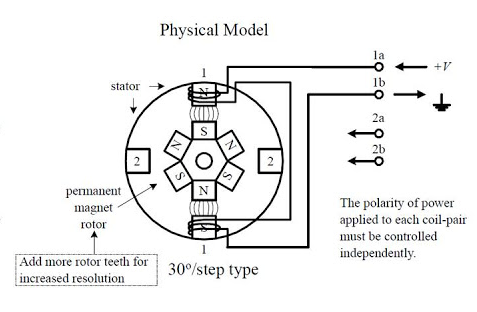
\includegraphics[width=\textwidth]{pics/bipolar_stepper.png}
	\caption{Need better / simpler figure here!}
	\label{fig:bipolarstepper}
\end{figure}

\subsubsection{Current Consumption}
%TODO values that calculate the current per motor?
%TODO ADD CURRENT MEASUREMENTS @ 2.2 v
The current consumed by a stepper motor is constant and independent of the angular velocity of the rotor.
The average current consumed is equal to: $\textrm{I} = V_{\text{supply}}/R_{\text{coil}}$.
Therefore running the motor at maximum speed, translates the most electrical energy into kinetic energy.
However, the motor speed is inversely proportional to the motor's output torque and therefore the maximum speed is limited by the minimal required output torque.
%The current trough the coils is constant, so the faster the stepper motor changes step the more energy can be transformed into movement.
%Increasing the rotational speed of the stepper motor decreases the torque output of the motor.
%Therefore the speed is limited by the amount of torque required to preform the movement.

\subsubsection{Control and Rotor Synchronization}

The only way to grantee that the teeth on the rotor will stay aligned with the coil, is to keep the coil energized until the next position is instructed and succeeding coil is energized. 
On the first startup the rotor may not be aligned with the last position in the sequence of four.
As a result an error between one and three steps can occur before the energized coil and rotor are synchronized.

In case the stepper motor is rotating and the power is removed, misalignment between the rotor and the last energized coil can occur.
While the rotor could be moving from one position to the next, it has not moved at all (undershoot) or can continue to move to the next position due to inertia of the rotating mass (overshoot). 
To determine what would be more likely, undershooting or overshooting, the following experiment has been preformed to determine the error in the number of steps.

\subsubsection{Experimental setup}

Tiny 6\,mm permanent magnet bipolar stepper motors from Nidec are frequently used in digital camera's~\cite{nidec_stepper_2017}.
For this motor one rotation is equal to 20 steps i.e five times the sequence of four.
This stepper motor is suspended and a needle glued to the motor shaft.
The needle rotates over a round piece of paper which is divided by markings in 20 steps.%, as seen from Figure \ref{fig:step_counting}.
First the rotor and coil are synchronized by moving four steps, and the position of the needle is visually recorded and written down.  
Then the stepper motor is commanded to make one rotation equal to 20 steps.
After rotating 20 steps the power is removed from the coils and the needle position is again visually recorded and written down.

\begin{figure}
	\centering
	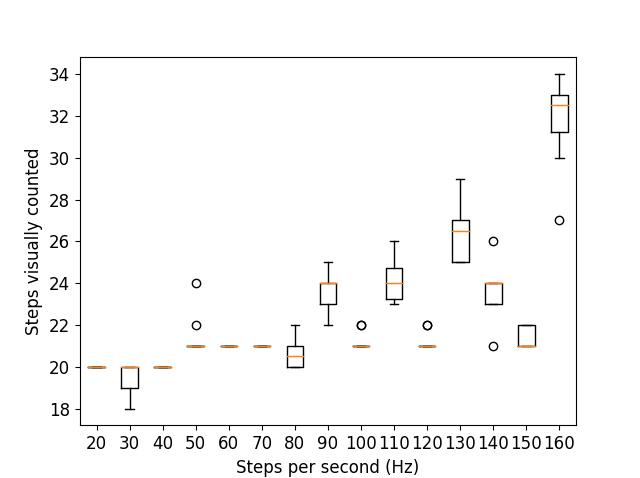
\includegraphics[width=0.8\textwidth]{pics/figure_intertia.png}
	\label{fig:step_results}
	\caption{}
\end{figure}


%\begin{subfigure}[b]{0.38\textwidth}
%	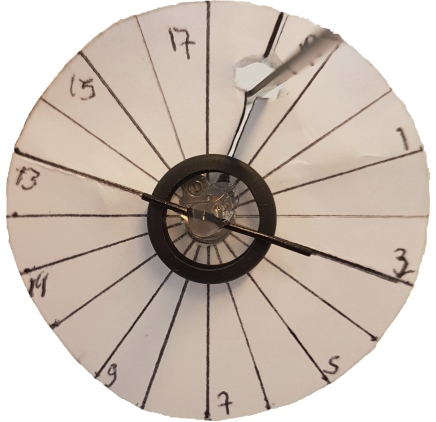
\includegraphics[width=\textwidth]{pics/step_counting.jpg}
%	\caption{Experimental setup for determining error in the number of counted steps}
%	\label{fig:step_counting}
%\end{subfigure}	


\subsubsection{Stepper Motor Inertia Result}

Figure \ref{fig:step_results} shows the result of the experiment.
The stepper motor on average will overshoot, i.e. will do more steps than commanded when the power is removed.
This effect is becomes more significant with increasing step frequency.
However, while this experiment only shows the effect for an unloaded motor, it is likely that a synchronization error will occur when a transiently-powered robot would be powered using two stepper motors in differential drive.
After every power interrupt each motor first needs to be synchronized, which will result in the robot making a random turn if the error between the motors is not equal.

\subsection{DC Motor locomotion}
\label{sec:pre_dc_motor_locomotion}
Small dc motors are commonly selected to provide locomotion for small robotic platforms as seen from Table \ref{tab:comparison_robot_platforms}.
In this section the DC motor will be evaluated as the locomotion type for the transiently-powered robot.

\subsubsection{Operation of a DC Motor}

When voltage is applied to the motor, current rises as quickly as the inductance in the motor windings allows.
DC motors produce an initial startup peak because the back electromotive force (back EMF) is initially zero.
The current reaches a maximum when the rotor starts to rotate and a back EMF is generated.
The back EMF will further increase while the motor accelerates to its steady state speed, and the speed is limited by the voltage supplied.

If a load is applied to the DC motor the current consumed by the motor is increased because current is proportional to the torque applied to the motor.
Additionally, the angular velocity of the motor will decrease while the torque is inversely proportional to the angular velocity of the motor.

\subsubsection{Evaluation of the Start Current Peak}
The DC motors used for robots are normally powered directly from the battery as linear or switch-mode power regulators are not able to supply the high start currents.
%In the worst case the start current peak can be equal to the stall current of the motor.
However, the use of a supercapacitor requires a regulator to make efficient use of the energy stored, as described in Section \ref{sec:pre_energy_harvesting_storage}.
The switch-mode regulator that is part of the BQ25570 energy harvester is only able to supply a peak output current of 110\,mA~\cite{bq25570_2017}.

%To evaluate the magnitude of the current peak, the free running current profile of 
The 206-11 DC motor from Precision Microdrives~\cite{gearmotor_206-110_2017} is the selected motor that will be evaluated.
From the datasheet a typical start current of 185\,mA can be found for its rated operating voltage of 3\,V.
However, the system voltage chosen for transiently-powered robot is 2.2\,V.
To determine the startup current of a 206-110 motor when supplied with 2.2\,V, a two second current trace is recorded using a Monsoon Power Monitor~\cite{monsoon_powermonitor_2017}.


\begin{figure}%[h!]
	\centering
	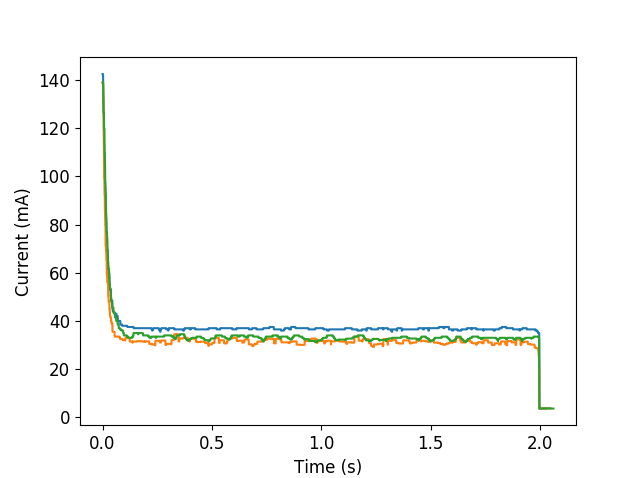
\includegraphics[width=0.62\textwidth]{pics/free_running_current.png}
	\caption{Current profile of the dc motor.}
	\label{fig:free_running_current}
\end{figure}

\subsubsection{Results}
The measurement results for three different motors is shown in Figure \ref{fig:free_running_current}
The results show that the 2.2\,V supply voltage reduces the start current peak to 140\,mA.
This is still above 110\,mA and the robot needs to power two motors in a differential drive configuration to allow steering.
A solution is to use pulse width modulation (PWM) to reduce the motor speed and average current consumed.
Combining PWM with a large bulk capacitor should enable the buck converter to start the motors.
However the PWM duty cycle will be limited to a maximum of $100/(2*140/110) = 39.2\%$, and will be further reduced by the load applied to the motors due to the weight of the robot.


\subsection{Conclusion}
Stepper motor can be categorized power hungry as this type of motor consumes a constant current independent of the rotational speed.
The only way retain rotor and stator stay alignment is by keeping the stepper motor coil energized.
Very frequent power interrupts could lead to loss of synchronization between the energized coil and position of the rotor as a result of rotor inertia.
The error due to inertia becomes more significant with increase rotational speed.
Loss of synchronization can result in random behavior of a differential drive robot, as one stepper motor may require a different amount of steps before synchronization than the other.

Alternatively a normal DC motors can be used which do not require any synchronization.
However, this motor requires a high start current which the buck converter from the harvester, might not be able to supply.
A big bulk capacitor can temporary supply high currents and PWM can be used to reduce the average current consumed by the motor.
Therefore the dc motor is chosen as the locomotion type used for the transiently-powered robot.

\section{Transiently-powered Robot Model}
\label{sec:transient_model}

In this section a simple model will be derived showing the relation between size and weight of the robot, the amount of power that is harvested and stored and how much of this can be translated into linear movement.

\subsection{Modeling Assumptions}

Energy is harvested from an ambient source and stored in a supercapacitor.
To make efficient use of the energy stored in a supercapacitor a regular is required to supply a stable voltage to the connected loads.
In this case the loads are two identical dc motors which each drive wheel. \\
\\ \noindent
The following assumptions will be used to model the transiently powered robot:
\begin{itemize}
	\item The required power by the loads is greater than the incoming power, resulting in repeated power cycling of the robot.
	\item The amount of input power after conversion is constant due to the use of a controlled environment
	\item Since a regulator is used, the voltage in the capacitor will never fall below the operating voltage.
\end{itemize}

%The input power Pin, will be stored in a supercapacitor with capacitance C.


%The regulated output voltage is a lower threshold for the energy that can be used from the capacitor.
%The upper threshold is determined by the maximum voltage rating of the supercapacitor.
%Lowering the output voltage allows for more energy to be used from the supercapacitor, and also lowers the overall power consumption of individual components.
%The energy stored in supercapacitor is a function of the capacitance and the threshold voltage difference, being equal to:








% 1 Incomming power V * I which scales with solar panel size

% 2 Maximum power point tracking (switchmode boost converter)

% 3 Stored in non-ideal supercapacitor with capcitiy C and a parrallel resistance Rleak and series resistance (ESR, typically small but not neglectable?)

% 123 determine chargetime

% Buck converter losses 

% Power consumed from source = Pcons = Ploss + Pweels

% Power P(t)  = F * v = T x omega

\subsection{Motor Dynamics}

The electrical equivalent circuit of a brushed dc motor is shown in Figure \ref{fig:pre_model_dc}, where $v$ is the voltage applied to the motor, $i$ the armature current, $R$ the armature resistance, $L$ the armature inductance, $e$ the back EMF voltage, $\tau$ the torque produced by the motor, $\omega$ the angular velocity of the rotor, $J$ is the moment of inertia of the rotor, $B$ is the viscous friction coefficient of the motor bearings and $m$ the external applied torque.


\begin{figure}[h!]
	\centering
	\begin{circuitikz}
		%\draw [help lines] (-1,-2) grid (12,5);
		
		% electrical equivalent circuit
		%\draw (0,0) to[V, v_=$v$] (0,3);
		\draw (0,3) node[ocirc] {}; % ,label=left:+
		\draw (0,3) to[R, i>^=$i$, l=$R$] (3,3);
		\draw (3,3) to[L, l=$L$] (4,3);
		
		\draw (0,2.25) node {$+$};
		\draw (0,1.5) node {$v$};
		\draw (0,0.75) node {$-$};
		
		\draw (4,3) -- (5,3);
		\draw (5,3) -- (5,2);
		%\draw (5,1.5) node[elmech](motor){M};
		\draw (5,1) -- (5,0);
		
		\draw (4.25,2.25) node {$+$};
		\draw (4.25,1.5) node {$e$};
		\draw (4.25,0.75) node {$-$};
		
		\draw (0,0) -- (5,0);
		\draw (0,0) node[ocirc] {}; 
		
		% motor
		\draw[fill=white] (4.85,0.85) rectangle (5.15,2.15);
		\draw[fill=white] (5,1.5) ellipse (.45 and .45);
		
		
		% shaft drive -> transmission
		\draw[fill=black] (5.45,1.45) rectangle (7.0,1.55);
		
		% momentum arrow of drive -> transmission
		\draw[line width=0.7pt,<-] (5.8,1) arc (-30:30:1);
		
		% moment of inertia
		\draw[fill=white] (7.5,1.59)
		ellipse (.15 and 0.4);
		\draw[fill=white, color=white] (6.9, 1.99)
		rectangle (8.49, 1.19);
		\draw (6.8,1.59) ellipse (.15 and 0.4);
		\draw (6.8,1.99) -- (7.5,1.99);
		\draw (6.8,1.19) -- (7.5,1.19);
		
		% momentum arrow (left hand side of brake shoe)
		\draw[line width=0.7pt,->] (8.05,1.1) arc (-30:30:1);
		
		% descriptions inside graphic
		\draw (5.85,2.2) node {$\omega_A, M_A$};
		\draw (7.25,1.61) node {$J$};
		\draw (8.05,2.32) node {$M_R$};
		
	\end{circuitikz}
	\caption{Brushed DC motor system model.}
	\label{fig:pre_model_dc}
\end{figure}

\noindent
Using Kirchhoff's voltage law the electrical dynamics of a dc motor can be described as
\begin{equation}
\label{eq:kirchhoff}
v = Ri + L \dot{i} + e
\end{equation}

\noindent
From Newton's second law follows that the mechanical dynamics of a motor can be described as
\begin{equation}
\label{eq:newton}
\tau = J\dot{\omega} + B\omega + m
\end{equation}

\noindent
The electromechanical equations state that the back EMF voltage is proportional to the angular velocity and the motor torque is proportional to the armature current

\begin{equation}
\label{eq:electomechanical}
\begin{gathered}
e = k_{e} \omega \\
\tau = k_{t} i
\end{gathered}
\end{equation}

\noindent
where $k_{e}$ is the back emf constant of the motor and $k_{i}$ the torque constant of the motor.
The electrical power consumed and mechanical power consumed will be equal to

\begin{equation}
\begin{gathered}
p_{\text{e}} = vi \\
p_{\text{m}} = \tau\omega
\end{gathered}
\end{equation}

\noindent
Rewriting equation \ref{eq:kirchhoff}, \ref{eq:newton} and \ref{eq:electomechanical} and appling the Lalace transa transfer function from $v$ to $\omega$ can be obtained, assuming $m$ = 0.

\begin{equation}
\frac{\Omega(s)}{V(s)} = \frac{k_{i}}{(Ls + R)(Js + B) + k_{\omega}k_{i}} 
\end{equation}

where $V(s)$ and $\Omega$ are the Lapace transformations from $v$ and $\omega$ respectively.


\subsection{Robot Dynamics}
The robot is modeled as a mass $m$, that is moved by two wheels with radius $r$, each connected directly to a motor.


The rolling friction between the wheels and the surface is equal to:
\begin{equation}
F_{\text{k}} = \mu_{\text{k}}mg
\end{equation}

Therefore the torque applied to the motor due to rolling friction, as it is only present while the robot is moving relative to the surface and the equation becomes:

\begin{equation}
T_{\text{ext}} = rF_{\text{k}} sgn(\omega)
\end{equation}

\noindent
The total mass is equal to the 